%%%%%%%%%%%%%%%%%%%%%%%%%%%%%%%%%%%%%%%%%%%%%%%%%%%%%%%%%%%%%%%%%%%%%%%%%%%%%%%%
%2345678901234567890123456789012345678901234567890123456789012345678901234567890
%        1         2         3         4         5         6         7         8

\documentclass[letterpaper, 10 pt, conference]{ieeeconf}  % Comment this line out if you need a4paper

%\documentclass[a4paper, 10pt, conference]{ieeeconf}      % Use this line for a4 paper

\IEEEoverridecommandlockouts                              % This command is only needed if 
                                                          % you want to use the \thanks command

\overrideIEEEmargins                                      % Needed to meet printer requirements.
\usepackage{graphicx}
\usepackage{amsmath}
\usepackage[hidelinks]{hyperref}
\usepackage{units}
%\usepackage{enumitem}
\newcommand{\M}[1]{\mathbf{#1}} % Bold for matrix
\newcommand{\V}[1]{\mathbf{#1}} % Bold for vector
%In case you encounter the following error:
%Error 1010 The PDF file may be corrupt (unable to open PDF file) OR
%Error 1000 An error occurred while parsing a contents stream. Unable to analyze the PDF file.
%This is a known problem with pdfLaTeX conversion filter. The file cannot be opened with acrobat reader
%Please use one of the alternatives below to circumvent this error by uncommenting one or the other
%\pdfobjcompresslevel=0
%\pdfminorversion=4

% See the \addtolength command later in the file to balance the column lengths
% on the last page of the document

% The following packages can be found on http:\\www.ctan.org
%\usepackage{graphics} % for pdf, bitmapped graphics files
%\usepackage{epsfig} % for postscript graphics files
%\usepackage{mathptmx} % assumes new font selection scheme installed
%\usepackage{times} % assumes new font selection scheme installed
%\usepackage{amsmath} % assumes amsmath package installed
%\usepackage{amssymb}  % assumes amsmath package installed

\title{\LARGE \bf
IMU-based pose-estimation for spherical robots with limited resources
}

\author{Jasper Zevering*, Anton Bredenbeck, Fabian Arzberger, Dorit Borrmann, Andreas Nuechter$^{1}$% <-this % stops a space
\thanks{*
        Corresponding author: }%
        \thanks{ \quad  \tt\small info@jasperzevering.de}%
\thanks{$^{1}$ All authors are with Informatics VII : Robotics and Telematics - University of Wuerzburg}%
\thanks{We acknowledge funding from the ESA Contract No. 4000130925/20/NL/GLC for the ``DAEDALUS -- Descent And Exploration in Deep Autonomy of Lava Underground Structures'' Open Space Innovation Platform (OSIP) lunar caves-system study and the Elite Network Bavaria (ENB) for providing funds for the academic program ``Satellite Technology''.}
}

\begin{document}



\maketitle
\thispagestyle{empty}
\pagestyle{empty}


%%%%%%%%%%%%%%%%%%%%%%%%%%%%%%%%%%%%%%%%%%%%%%%%%%%%%%%%%%%%%%%%%%%%%%%%%%%%%%%%
\begin{abstract}

Spherical robots are a robot format that is not yet thoroughly studied for the application of mobile mapping.
However, in contrast to other forms, they provide some unique advantages.
For one, the spherical shell provides protection against harsh environments, e.g., guarding the sensors and actuators against dust and solid rock.
This is particularly useful in space applications. 
Furthermore, the inherent rotation the robot uses for locomotion can be exploited to measure in all directions without having the sensor itself actuated.
A reasonable estimation of the robot pose is required to exploit this rotation in combination with sensor data to create a consistent environment map. 
This raises the need for interpolating instances for calculation-intensive slow algorithms such as optical localization algorithms or as an initial estimate for subsequent simultaneous localization and mapping (SLAM).
In such cases,  inertial measurements from sensors such as accelerometers and gyroscopes generate a pose estimate for these interpolation steps.

The paper presents a pose estimation procedure based on inertial measurements, that exploits the known dynamics of a spherical robot. 
It emphasizes a low jitter to maintain constant world measurements during standstill and avoids exponentially growing error in position estimates. 
Evaluating the position and orientation estimates with given ground truth frames shows that we reduce the jitter in orientation and handle slip and partly slide behavior better than other commonly used filters such as the Madgwick filter.

\end{abstract}


%%%%%%%%%%%%%%%%%%%%%%%%%%%%%%%%%%%%%%%%%%%%%%%%%%%%%%%%%%%%%%%%%%%%%%%%%%%%%%%%
\section{INTRODUCTION}


Spherical robots are a relatively narrow field of robotics. Still, they could be useful in situations where the measurement equipment needs to be protected against harsh environments.
As an example, the 2021 CDF study LunarCaves by ESA about the feasibility of a spherical robot, called DAEDALUS, for exploration of lunar-lava tubes \cite{rossi2021daedalus} shows the need for orientation and position estimation of spherical robots with the limitations on resources common for space-applications.
Although a purely Inertial Measurement Unit (IMU)-based estimation is not recommended for various reasons, the lack of an absolute reference among others, IMU-based pose estimation is used as part of an overall multi-sensor-fusion-based estimation.
IMUs are sensors with higher refresh rates than Simultaneous Localization and Mapping (SLAM) based algorithms, such as optical or Light Detection and Ranging (LIDAR) SLAM. This makes them suitable for interpolating the more precise and absolute position reference points of these slower algorithms.
The limited computational power of space-qualified CPUs further imposes the need for good orientation estimation without computational-intensive algorithms like Kalman filters.
Lastly, the geometry of a spherical robot opens the possibility for the not often used position estimation by IMUs.

This paper introduces an IMU-based orientation and position algorithm for spherical robots with limited computational power and the need for real-time estimations.
The algorithm does not rely on one specific locomotion approach, but it assumes a rotation of the IMU together with at least the shell of the robot, if not the whole robot. 
The experiments in this paper use the setup of the IMUs of the prototype depicted in Figure \ref{fig:prototype}, which is inspired by previous work such as Daedalus \cite{rossi2021daedalus}.
Due to the lack of a locomotion system, the sphere needs to be rolled externally. 
A Livox Mid-100 laser scanner was used for evaluation purposes.
In addition to analying the filtered output the evaluation will show and discuss the resulting point clouds of this prototype with the presented pose estimation.
\begin{figure}[b]
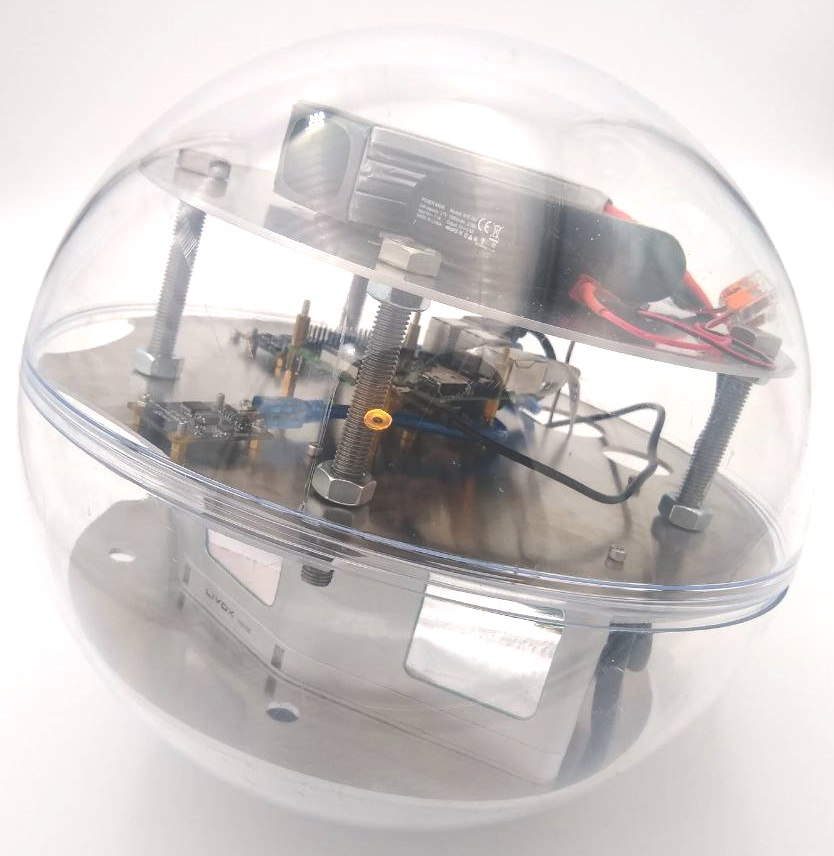
\includegraphics[width=0.49\linewidth]{./graphics/photoReal1.jpeg}
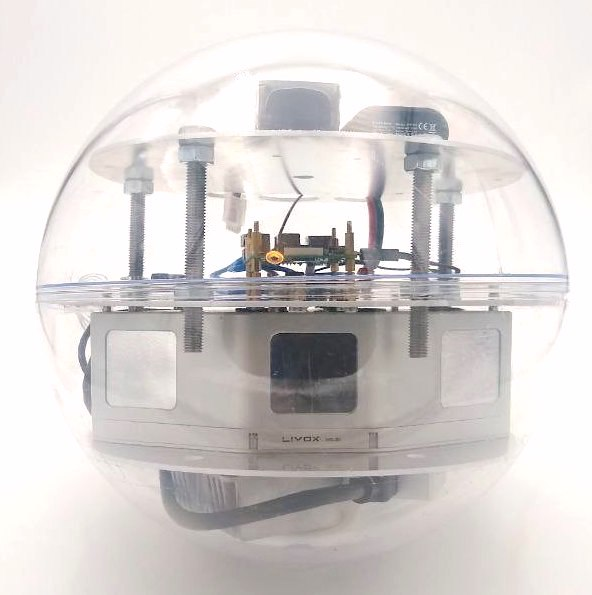
\includegraphics[width=0.50\linewidth]{./graphics/photoReal3.jpeg}
\caption{Prototype to test the algorithm in an envisaged technical environment. The main payload is the Livox Mid-100 laser-scanner. For pose-estimation, three IMUs of the manufacturer Phidget are placed on the middle plate and a Raspberry Pi 4 for the calculations. On the top are two batteries and on the bottom one voltage stabilizer and breakout box of the laser-scanner. }
\label{fig:prototype}
\end{figure}


\section{Assumptions and Prelimitations}
\label{sec:AssumptionsAndPrelimitations}
The presented approach works for any spherical robot with IMUs that moves based on rotation.
Nevertheless, it requires multiple assumptions to be beneficial in comparison to existing approaches.
Some of these arise from the fundamental behavior of spherical robots and some more specific from the DAEDALUS project.
The approach becomes beneficial given the following assumptions and requirements:

\paragraph*{1. Real Time Operations}The operation of the robot requires real time calculation of the pose. This implies the usage of onboard computational power.
\paragraph*{2. Limitation of Computational Power}
Due to the need for efficient code without massive bottleneck operations, such as matrix inversion in the extended Kalman Filter, the code must minimize the usage of non-basic operations.
\paragraph*{3. Low Costs of Hardware}
We assume biased and noisy data in a non-negligible amount from the sensors.
\paragraph*{4. Sphere Shape}
The code relies heavily on the assumption of a spherical shape with a constant radius. Accordingly, rotation on the ground leads to translation.
\paragraph*{5. Slip and Sliding}
We assume the sphere is affected by both slip, i.e., the sphere rotates with no resulting translation, and sliding, i.e., the sphere may translate without rotating in a limited, non-permanent way. The limitation refers to the assumption that sliding and slipping reduce the amount of translation for a given rotation and vice versa, however, not for complete absence.
\paragraph*{6. Stability of Pose}
For SLAM purposes using LIDARs, a stable but maybe minimal false pose is preferred over a more exact but noisy and jumping position.
\paragraph*{7. Further Processing of Pose}
The approach should avoid jumping values or abrupt changes of data if not clearly indicated by the sensors. Suppose there is an internal algorithmic change of behavior due to the change of state from standing to rolling. This change shall not be represented by an unnatural acceleration in the data.
\paragraph*{8. Uncertainty of Iterative Position Integration}
IMUs deliver no absolute reference for a position as they do for orientation in the form of a noisy but measurable gravity vector. So without external or secondary sensors relying on absolute waypoints, the position estimation will always underlie the integration of errors.
\paragraph*{9. Space Suitability}
As the algorithm is considered to be applied for space missions, the magnetometer data is not considered in the algorithm, despite its positive impact on orientation estimation on Earth.
\paragraph*{10. Short Term Mobility}
The approach is targeted at a spherical robot for data collection with a laser scanner, requiring standstill periods for scanning.
In further extension, the fusion of a pose estimation by the laser scanner will be merged.
Thus, the sphere is considered to move in multiple short paths and not roll continuously for a long perod.
Relying on integration parts, the IMU-based algorithm benefits from this assumption.
\paragraph*{11. Non-reliability of locomotion commands}
For DAEDALUS, the same input of the locomotion controller leads to heavily different behaviors depending on the pose of the robot and the surface structure \cite{rossi2021daedalus}.
Also, the DAEDALUS robot has two utterly different locomotion methods; therefore, we will not take locomotion itself, nor the controller input or output into account for pose estimation.



We conclude that the generated data has to be a compromise between simple on-board filtration of data, while still being usable for heavy calculation post-record, e.g. map generation.
It has to be easy to calculate and adapt to the specific needs.
Making assumptions about the dynamics of the system, it must nevertheless deliver reliable estimates which take physical behavior into account.
It shall be real-time capable and does not rely on delayed steps.
The resulting algorithm is restricted to spherical or cylindrical robots. 
It is optimized for gathering laser data where noisy pose estimates while standing deteriorate the map creation process, and therefore, even if slightly false, a stable position is preferred.

\section{State of the Art}
\label{sec:SOA}
For pose estimation on embedded hardware, there are three main algorithms.
\subsection{Kalman Filter}
The Kalman Filter or the more suitable Extended Kalman Filter (EKF) use state prediction and correction based on sensor data for orientation estimation \cite{Kalman1960}.
For the defined limitations, the Kalman Filter is not suitable.
First, the EKF requires a considerable amount of computational power, mainly due to matrix inversion. For this, the needed calculations grow exponentially with input data.
Further, the Kalman Filter relies on input to a system to calculate an estimation of the pose for the next iterative step.
But, as described in Section \ref{sec:AssumptionsAndPrelimitations}, we cannot take the input to locomotion control as a reference for pose estimation as the behavior is not linear or even predictable without exact knowledge of the surface.
Therefore it is not possible to implement a physical behavior of the system to the filter, as easily as it is for other robotic applications.
The Error State Extended Kalman Filter, which works solely with IMU data \cite{ahmadi2007orientation}, requires substantial computational power.
For the later introduced position estimation for spherical robots, some calculations are used for the orientation as well as for the position.
After all, if computational power is not limited, Kalman Filters provide principally better results.
\subsection{Madgwick Filter}
The Madgwick filter is a widely used filter for orientation estimation with IMUs \cite{madgwick2010}.
It is efficient and easy to calculate but does not consider the physics of the motion.
It uses a gradient descent algorithm.
It nearly provides the sought-after classification for the orientation.
The behavior is shown in comparison to the complementary filter in Figure~\ref{madgVsComp1}.
Being optimized for movement the Madgwick filter has a jittering behavior at the standstill of the IMU.
This does not meet the desired behavior as described in the prelimitations Section~(\ref{sec:AssumptionsAndPrelimitations}).
As we do not use a magnetometer, we cannot use the gyro bias estimation of the Madgwick filter.
\subsection{Complementary Filter}
A complementary filter is a fundamental approach of combining precise but not exact with non-precise but exact data.
Therefore it is widely used for combining noisy accelerometer data with gravity as a reference with the precise but drifting measurement of gyroscopes.
The basic concept is to have the main part of a value dominated by a gyroscope but, over time, a slow drift towards the measurement of the accelerometer.
E.g., for pitch, this results in 
\begin{equation}
\theta_n = (1-\alpha) \cdot (\theta_{n-1}+ \Delta\theta_{gyro})+ \alpha \cdot \theta_{acc},
\end{equation}
where $\alpha$ is the complementary gain. 
It determines how much weight the accelerometer data gets and how fast the value drifts towards the measurement of the accelerometer.
Therefore the gyroscope functions as high-pass and the accelerometer as low-pass part of the basic complementary filter \cite{min2015complementary}.
A commonly used value for $\alpha$ is 0.02, meaning every iteration, 2 percent of the new values come from the accelerometer.
This corresponds, with the used \unit{125}[Hz] calculation, to frequency-border of the low and high-pass  of \unit{2.5}[Hz] \cite{hajdu2017complementary}.
With $\alpha=1$ the result is the accelerometer data and the gyroscope has no influence. \\
The complementary filter is best for orientation calculation without position change as the accelerometer value relies on calculating the gravity value.
Acceleration in one direction leads to a miscalculation of the gravitational vector and therefore false orientation estimates.
Simple orientation estimations of quadrocopters often change the $\alpha$ gain to 0 while moving to avoid the miscalculation of the gravity vector \cite{mahony2005complementary}.



\begin{figure}
%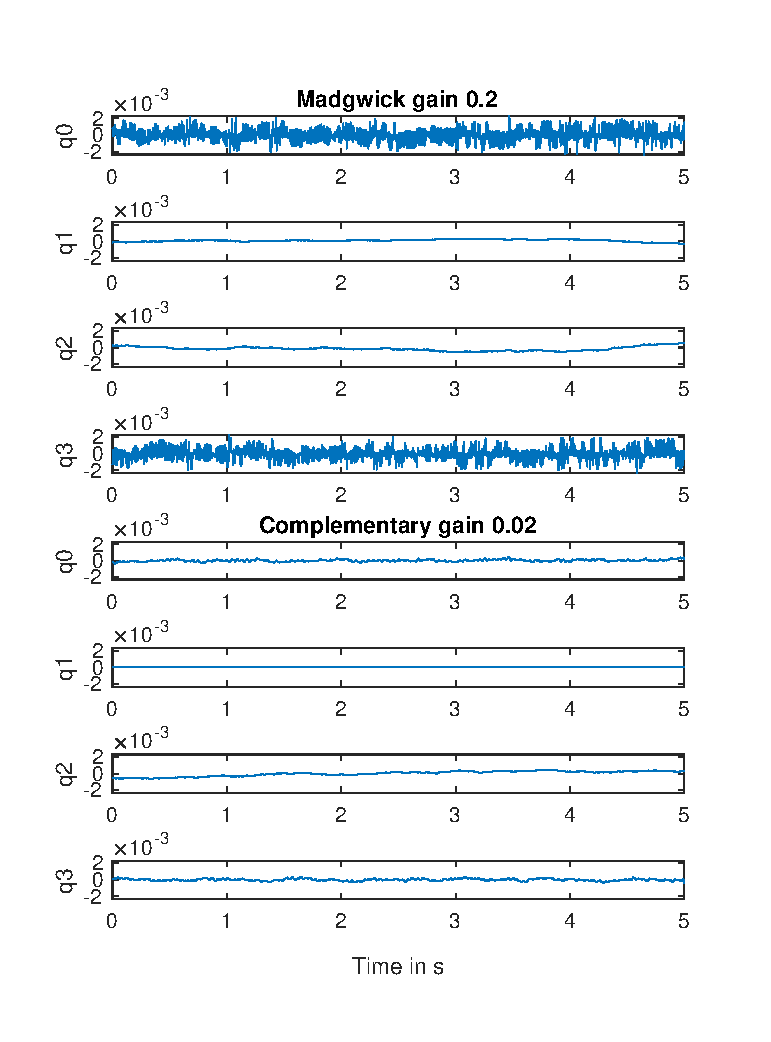
\includegraphics[width=\linewidth]{./graphics/MadgwickVsComplementaryNoMovement.eps}
\makebox[\linewidth][c]{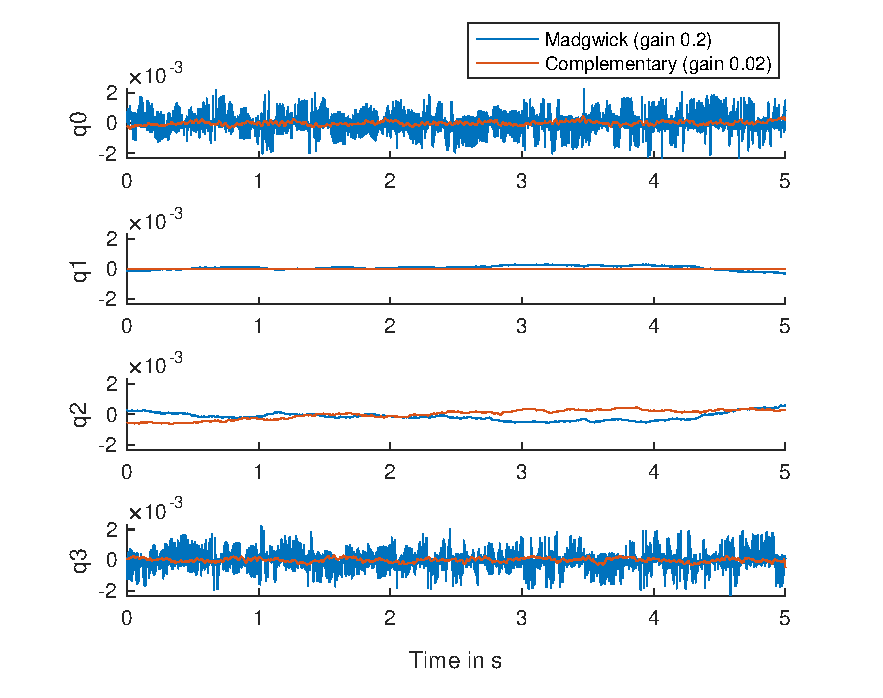
\includegraphics[width=1.15\linewidth]{./graphics/CompelemntaryVsMadgwick6seconds.eps}}
\caption{Quaternion values of Madgwick filter and complementary filter with default gains when IMU is at a standstill. The Madgwick filter has clearly visible jitter, the complementary filter has not.}
\label{madgVsComp1}
\end{figure}



\subsection{Position Estimation}
Position estimation purely by IMU is not recommended as the double integration of the accelerometer measurements leads to exponential error summation \cite{thong2004numerical}.
Therefore there are very few approaches targeting this way of position calculation \cite{kok2017IMU}.
The very impressive work in \cite{valencia2017simpleIMU} also uses IMUs for 6D pose estimation.
They follow a pre-specified trajectory with a manipulator and manage to estimate its pose within 10\% of the ground truth.
Given their application is rather broad, they do not exploit known dynamics of the system, which could be helpful for spherical robots.


\section{Filter-concept}
The pose estimation for spherical robots is a concept with interconnected components.
Both orientation and position estimates are computed based on gyroscope and accelerometer measurements, taking into account the limitations of the system described in Section \ref{sec:AssumptionsAndPrelimitations}.
The generalized overview of orientation and position estimation is shown in Figure \ref{generalized}.

\begin{figure}%[hb]
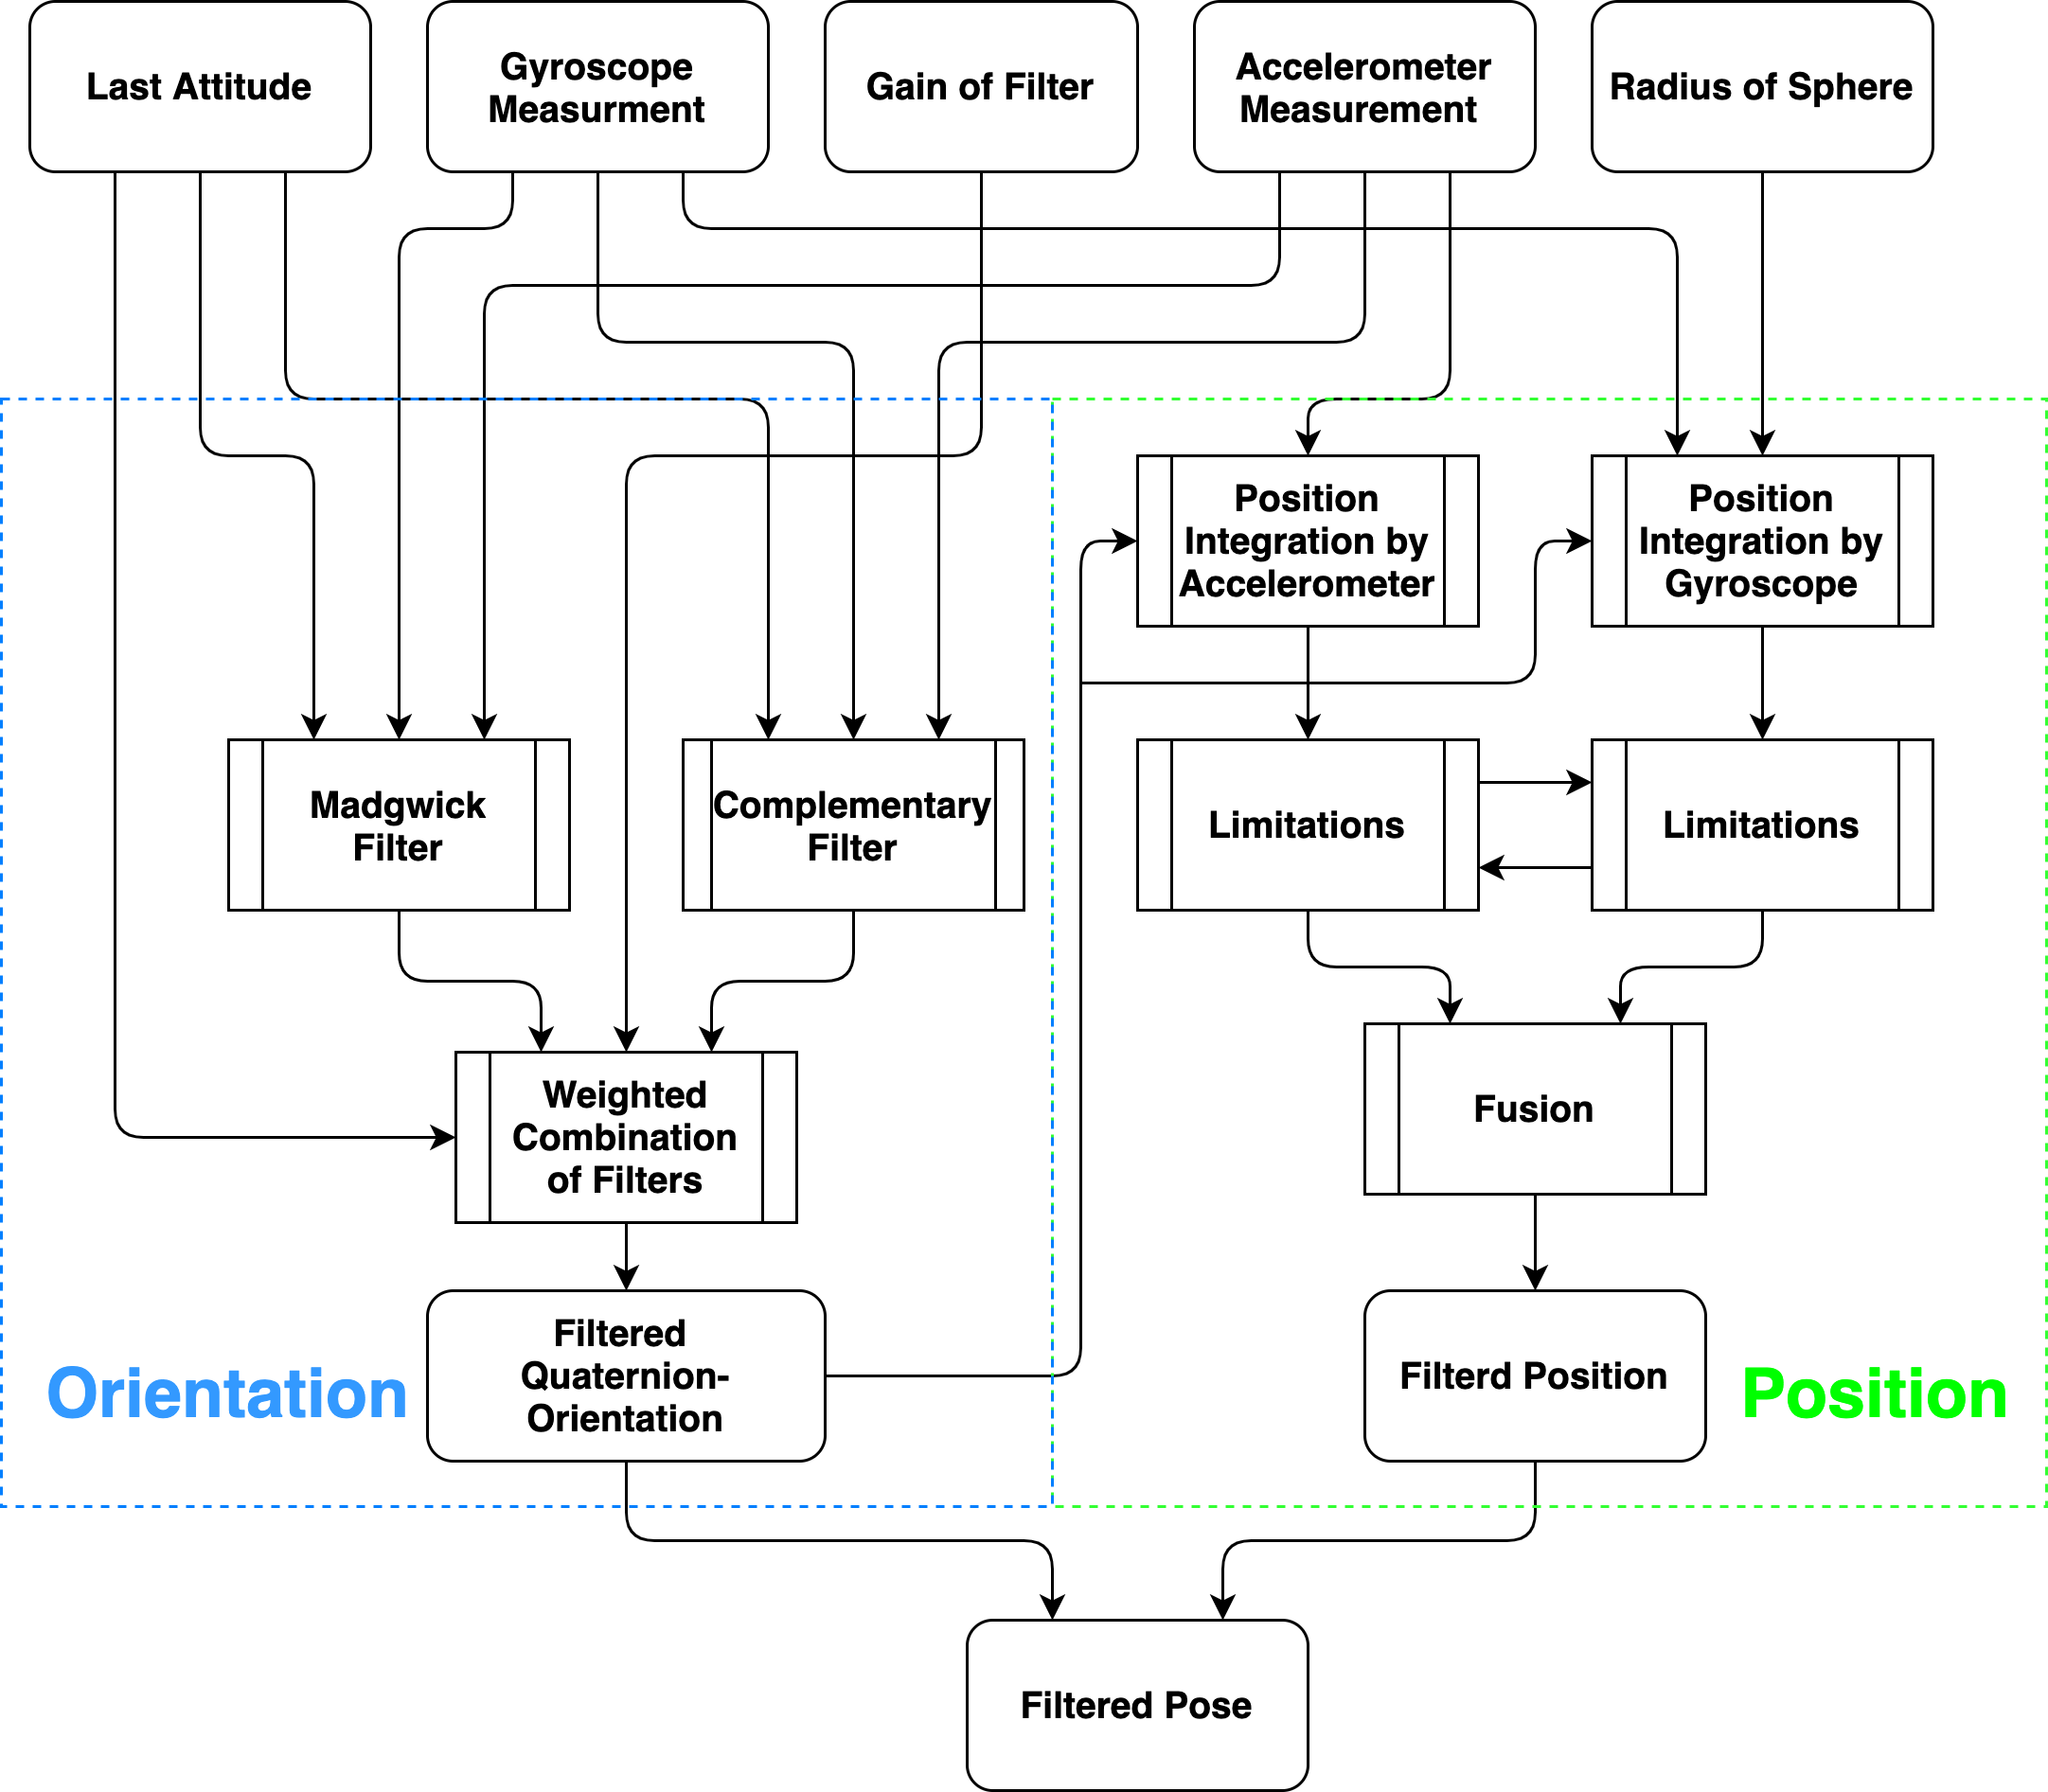
\includegraphics[width=\linewidth]{./graphics/imuJasperChartSimliefiedBIG.png}
\caption{Diagram of the estimation.}
\label{generalized}
\end{figure}


\subsection{Orientation}
The orientation estimation is the combination of the Madgwick and a complementary filter.
The weaknesses and strengths of both described in Section \ref{sec:SOA} are combined. 
The general idea is to distinguish between motion and standstill.
In motion the Madgwick filter is used and without motion the complementary filter.
This approach of distinguishing the evaluation algorithm depending on the state of motion of a robot has been done before, like in \cite{Hertzberg2012}.
The transition needs to be in a differentiable way, as this is one of our limitations.  
As both filters are applied with weights, this is done by an allocation of a given gain towards one or the other filter depending on the likelihood the sphere is moving or standing still. 
Therefore, this requires an adapting mechanism and an estimation of how likely the sphere is to rotate and hence translate.
Both filters share the same meaning of the gain, describing the influence of the accelerometer on the orientation.
The Madgwick filter weight determines how much influence the accelerometer measurement has on the overall orientation, just in a different way than the complementary filter.
Thus the implementation of this approach does not endanger the stability of the estimation due to the change between two completely independent approaches.
The algorithm can shift the gain from one filter to the other in a smooth way without jumping values or abruptly changing behavior. 

\subsection{Position}
As there is no absolute reference of position neither with calculation by gyroscope nor by the accelerometer, the filter can only try to improve the calculation of the velocity leading to the change in position. 
The straightforward approach is to double integrate the accelerometer, which leads to the earlier described unwanted behavior of exponential error integration and makes the position estimates completely unusable. 

An alternative approach multiplies the rotation speed with the known radius of the sphere and takes this as velocity, integrating once.
The more precise and less noisy data of the gyroscope leads to usable position estimates. 
There is no such extensive error integration, and more importantly: no exponentially growing error with time. However, if the sphere slips, this approach will predict the full translation.
Also, if there is translation but just slight rotation because of sliding, it will predict too little translation. 
Furthermore, integrating the rotation does not let us estimate vertical movement.
Thus, this approach neglects potential slip and sliding (limitation 5) as well as vertical movement. 
Every rotation will be predicted as translation in a given plane, which is most likely parallel to the ground. 
For instance, if the sphere rolls up an obstacle, the length of the path is estimated to be the ground-plane.

Our algorithm combines both approaches of position estimation and limits all components according to the other components. 
This implies a connection between translation and rotation. 
Overall the extreme situation (full translation, no rotation, or the other way round) will automatically lead to wrong predictions, as there is no way to tell which of the two approaches has at that moment more reliable data.
Therefore, the combination of both rather than only one is chosen.


\section{Filter-Implementation}

\subsection{Orientation}
The orientation is a symbiosis of the Madgwick filter and complementary filter. The complementary filter is chosen for no or slow motion, the Madgwick filter for fast motion. The Madgwick filter itself is untouched.
The standard complimentary filter works with Euler angles (roll, pitch, yaw (RPY)) resulting from the direct integration of the gyroscope while the Madgwick filter outputs quaternions.
Quaternions were designed under the premise of being free from singularities, i.e., for a continuous change in orientation, there exists a continuous change in quaternion representation \cite{becker2017dealing}. 
This is not the case for Euler angles, as a transition of a 359-degree roll to a 0-degree roll has no continuous value representation if limited to 360 degrees.
Updating the orientation for the complementary filter implies a transition of each angle independently.
Combining both representations leads to contradicting updates from each filter with respect to the other.
Thus, the complementary filter is adapted to work in quaternion representation.
%\begin{equation}
%\begin{bmatrix}
%\Phi_{new} \\
%\theta_{new}\\
%\Psi_{new}
%\end{bmatrix}
%= (1-\alpha)\begin{bmatrix}
%\Phi_{old} \\
%\theta_{old}\\
%\Psi_{old}
%\end{bmatrix}
% + \alpha \begin{bmatrix}
%\Phi_{acc} \\
%\theta_{acc}\\
%\Psi_{acc}
%\end{bmatrix}
%\end{equation}
Hence, the RPY-orientation is transformed to a quaternion, and then a quaternion slerp is performed \cite{dam1998quaternions}.
 The quaternion slerp utilizes the representation of two quaternions on a sphere. The transition from one quaternion to the other is not done directly but always over the surface of the sphere.
 This leads to the same handling of quaternions as the Madgwick-filter without endangering robustness due to using two different quaternions with very different values representing nearly the same position.
 
The transition between the two filters is done by shifting a fixed factor among the $\alpha$-gain of the complementary filter and the gain factor of the Madgwick filter.
 As the common values widely used for both values differ by one order of magnitude, the gain shifted to the complementary filter is divided by ten and the other way around.
 The values of the gyroscope axes determine in which manner to shift the overall gain to both filters. 
 The defining values are the two thresholds for using solely the complementary filter on the one hand or a full Madgwick filter on the other hand. 
 These values have been determined empirically.
 Future work will investigate improving those values by developing a suitable heuristic for the thresholds.
 The transition between the full complementary and the full Madgwick estimation, as is required by the prelimitations,  can be done by a function suitable for the specific scenario.
 This avoids large accelerations of the orientation due to the rapid change from one algorithm to another.
 In our experiments, when starting from standstill, the incipient Madgwick filter has a more rapid impact on the orientation values than the incipient complementary filter when stopping rotation. 
Therefore the transition between $\alpha$-gain of the complementary filter and the Madgwick-gain was chosen to have quadratic behavior. 
The value referred to as autogain $\Theta$ indicates how much impact both employed filters have on the orientation estimation. 
Therefore we calculate factors from the gyroscope measurements and scale the autogain with the maximum $\beta$ (cf. equation \ref{eq:factors} and \ref{eq:weight_autogain}).
$g_{k}$ represents the gyro measurement in the corresponding axis $k$, in rad/s. Later on, these factors will again be used for position estimation, namely to determine if the sphere rotates or not.
These factors are heuristically defined as:

\begin{equation}
f_k =
\left\{
\begin{aligned}
0& & g_k \leq 0.1  \\ 
0.25\cdot (g_x&-0.1)^2& \quad 0.1< g_k <2.1 \\
 1& & g_k \geq 2.1
\end{aligned}
\label{eq:factors}
\right. ,
\end{equation}

\begin{align}
\beta &= \max(f_x,f_y,f_z).\label{eq:weight_autogain}\\
\intertext{Then the Madgwick gain $\gamma$ for a given autogain $\Theta$ is calculated by} 
\gamma &= \Theta \cdot \beta. \\
\intertext{The complementary filter gain $\alpha$ is calculated by}
\alpha &= \Theta \cdot \theta \cdot(1-\beta).
\end{align}
Thus, the Madgwick gain has a maximum of $\Theta$ and $\alpha$ a maximum of $\theta\cdot \Theta$. This ratio $\theta$ can be adapted to specific needs.
We used $\theta = 0.1$ as the ratio between the two often used standard values $\gamma = 0.2$ and $\alpha= 0.02$.
Hence for adapting the position estimation to a given robot, the function for calculating the factors needs to be adapted in such a way that it is a good indication for movement or standstill.
The ratio $\theta$ needs to be chosen in a way that the desired ratio between Madgwick and complementary gain is reached.
And lastly, the autogain needs to be chosen to fit the specific needs in terms of how strong both filters should be able to influence the orientation.
We used $\Theta = 0.2$ to get the described common values.


\subsection{Position}
The calculated orientation is directly used for position calculation.
With the orientation, a gravity vector is calculated, which, once normalized, represents the measurement of the accelerometer in abstinence of movement. 
Let $\V g=\begin{bmatrix}0 &0 & -1 \end{bmatrix}^T$ represent the gravity vector in the world frame and the matrix $\M R$ represent the current orientation of the IMU, then


\begin{equation}
\V g\V '=\begin{bmatrix}
g'_x\\
g'_y\\
g'_z
\end{bmatrix}
= \M R \cdot \begin{bmatrix}
0 \\0  \\ - 1
\end{bmatrix}
\end{equation}
describes the effect of gravity in the coordinate system of the IMU.
This gravity vector is then subtracted from the accelerometer measurement. If there is no translation, the subtraction should lead to $\begin{bmatrix}
0 & 0&0
\end{bmatrix}^T$ meaning there is no acceleration other than gravity. If there are non-zero components, there is an acceleration in that direction. Given the accelerometer measurement $\V a$ this leads to the velocity vector
\begin{equation}
\begin{bmatrix}
v_{x\text{Acc}} \\ v_{y\text{Acc}} \\v_{z\text{Acc}} 
\end{bmatrix}
= 
\int_0^T \left(\begin{bmatrix}
a_x \\ a_y \\ a_z
\end{bmatrix} 
-  \begin{bmatrix}
g'_x\\
g'_y\\
g'_z
\end{bmatrix} \right)\, dt.
\end{equation}
These values are now coupled to the rotation of both axes other than their own.
Therefore, the factors from the orientation step, representing the likelihood of rotation, are used as limiting factors:
%TODO So würde man das programmieren, aber mathematisch ist das nicht korrekt.
\begin{equation}
\begin{bmatrix}
v_{x\text{AccL}} \\ v_{y\text{AccL}} \\v_{z\text{AccL}} 
\end{bmatrix}
 = \begin{bmatrix}
v_{x\text{Acc}} \\ v_{y\text{Acc}} \\v_{z\text{Acc}} 
\end{bmatrix}  \cdot 
\begin{bmatrix}
\max(f_y, f_z) \\ \max(f_x, f_z) \\ \max(f_x, f_y) 
\end{bmatrix}.
\end{equation}
If one of the three factors is 1, this means there is a translation in this direction.
When there is no rotation, it will set the velocity to 0.
During fast motion, this allows exponential error integration. 
This exponential error is taken care of later on.

The rotation into the world frame is computed as:
\begin{align}
\begin{bmatrix}
v_{x\text{\text{AccWorld}}} \\ v_{y\text{AccWorld}} \\v_{z\text{AccWorld}} 
\end{bmatrix}
&= \M R^T \cdot \begin{bmatrix}
v_{x\text{AccL}} \\ v_{y\text{AccL}} \\v_{z\text{AccL}} 
\end{bmatrix}.
\intertext{The next step requires the velocity calculated by the rotation.
Therefore the rotations (direct values from the gyro) are rotated into the world frame:}
\begin{bmatrix}
\omega_{x\text{World}} \\ \omega_{y\text{World}} \\(\omega_{z\text{World}}) 
\end{bmatrix} &= 
 \M R^T \cdot
\begin{bmatrix}
g_x \\ g_y\\ g_z
\end{bmatrix}. 
\end{align}
The rotation around the world $z$-axis is not used to calculate the velocity.
Its effect on the position is considered when determining the orientation in the world coordinate system.
$\omega_{z\text{world}}$ does not need to be computed as it has no influence on the position.


The resulting velocities are calculated by multiplying the circumference of the sphere:
\begin{equation}
\begin{bmatrix}
v_{xz\text{GyroWorld}} \\ v_{yz\text{GyroWorld}}
\end{bmatrix} = 
\begin{bmatrix}
\omega_{y\text{World}}/(2 \pi ) \\ \omega_{x\text{World}} / (2 \pi)
\end{bmatrix}
\cdot 2\pi r = \begin{bmatrix}
\omega_{y\text{World}}\\ \omega_{x\text{World}} 
\end{bmatrix}
\cdot r \,,
\end{equation}
where $r$ is the radius of the sphere.
As the gyro measures rad/s the value is divided by $2\pi$.
Note that the two-dimensional velocities $v_{xz\text{GyroWorld}}$ and $v_{zz\text{GyroWorld}}$ do not correspond to the velocity on the ground plane but may consist of motion in $z$ direction. 

 
 Next, the $v_{x\text{AccWorld}} $ and $v_{y\text{AccWorld}} $ are limited depending on $v_{xz\text{GyroWorld}} $ and $ v_{yz\text{GyroWorld}}$. In our experiments, this was 120 percent of the gyro calculated velocity.
 This ensures no exponential error integration when in motion.
 This is coupled to the physical act of sliding.
 The higher the likelihood of sliding, the higher the velocity should be compared to the velocity based on rotation.
 This does not count for slipping, as this implies the adaption of limitation of the velocity by rotation by the velocity measured by the accelerometer.
 But there is no need for a limitation as there is no double integration with the rotation.\\
 The last step for calculating the velocity is taking the velocity in $z$-direction into account for the velocity by rotation.
 This velocity in $z$ is from the noisy double integration, as this is the only indication for change of the $z$-axis.
 To avoid large errors and unlimited double error integration, $v_{z\text{AccWorld}} $ is limited to the mean of $v_{xz\text{GyroWorld}} $ and $ v_{yz\text{GyroWorld}}$.
With the Pythagorean theorem the velocity in $x$ and $y$ is calculated accepting the velocity in $z$-direction, which cannot be derived by the velocity from gyro:
 \begin{equation}
\begin{bmatrix}
v_{x\text{GyroWorld}} \\ v_{y\text{GyroWorld}}
\end{bmatrix} = 
\begin{bmatrix}
\sqrt{v_{xz\text{GyroWorld}}^2-v_{z\text{AccWorld}}^2}  \\ \sqrt{v_{yz\text{GyroWorld}}^2-v_{z\text{AccWorld}}^2 } 
\end{bmatrix}.
\end{equation}
The last step to get the position is the integration of the velocity:
\begin{equation}
\begin{bmatrix}
p_x \\ p_y \\p_z
\end{bmatrix}
 = \int_0^T \begin{bmatrix}
 (1-\beta)v_{x\text{AccWorld}} + \beta \cdot v_{x\text{GyroWorld}} 
 \\
  (1-\beta)v_{y\text{AccWorld}} + \beta \cdot v_{y\text{GyroWorld}} 
 \\
 v_{z\text{AccWorld}} 
 \end{bmatrix} dt.
\end{equation}
Depending on the practical circumstances and quality of measurement, the factor $\beta$ determines whether the position relies more on the accelerometer calculated velocity or the gyro.
There should always be a mixture of both if there is slipping and sliding.
$\beta =0.5$  results in the mean of both approaches.

\subsection{Time Complexity}

Overall a pose estimation step consists only of operations that are constant in time. 
Given that we use the fast inverse square root algorithm \cite{FastInvSqrt} for normalization, the trigonometric functions are considered the remaining bottleneck.
Overall there are 14 trigonometric function calls ($4\times \arctan$, $4\times\sin$, $4\times\cos$, $1\times \arcsin$, $1\times\arccos$) and $5$ divisions. 
The IMU measurements are collected at \unit[125]{Hz} and are processed without problems on a raspberry pi.
Hence no overwhelming computational load is to be expected.

 
 

\section{Evaluation}
The proposed algorithm is evaluated by two sets of experiments performed with three Phidgets 3/3/3 IMUs mounted on a circular acrylic glass plate with a diameter of \unit[29]{cm}.
For position experiments, the plate is put inside an acrylic glass sphere with the same radius as the glass plate.
First, the fusion of Madgwick and complementary filter, here denoted as Autogain, is compared to a Madgwick only estimate. Second, the trajectory computation using both gyroscope and accelerometer is evaluated.

\subsection{Orientation}
A first experiment is performed to show the overall performance of the Autogain computation for the orientation. The IMU was manually rotated in arbitrary directions, and the orientation was plotted using the Madgwick filter and the Autogain filter.
As expected, the overall behavior of the presented algorithm and the Madgwick filter is very similar in the dynamic case, as shown in Figure \ref{quaternion1}.
\begin{figure}
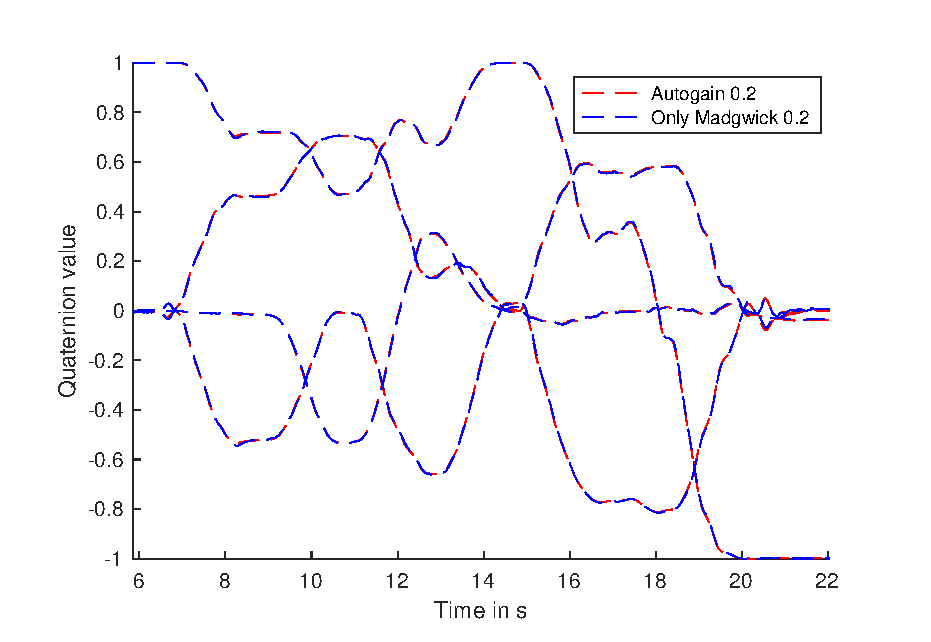
\includegraphics[width=\linewidth]{./graphics/AutoVsMad.eps}
\caption{Quaternion-values of the presented fusion of complementary and Madgwick filter and only the Madgwick filter.}
\label{quaternion1}
\end{figure}
The more expressive part is the change between motion and standstill, as in motion, both filters use the same algorithm but differ during standstill and slow motion.
As described in Section \ref{sec:SOA}, the Madgwick filter has a rather strong jitter during slow movements and standstill. 
This is due to the (too) large steps of gradient descent iterations.
To compensate for this, one needs to lower the gain, leading to more imprecise results during movement, as large iteration steps are beneficial there.
Alternatively, one needs to increase calculation frequency, which is in our scenarios limited by the hardware capabilities of the IMU.


To evaluate specifically the change between slow motion and standstill, a further experiment is performed.
Figure \ref{distance} shows the distance to a precise external reference over a short excerpt of the experiment with three phases of slow motion and rotation at second 7, 9 and 11. 
For external reference, we used a precise optical tracking system. 
The definition and proposed calculation of the distance of 2 quaternions of \cite{kuffner2004effectiveDistance} was used.
It describes the direct angle between two quaternions.
The optical system matches the overall orientation of both IMU-based algorithms quite well and lacks the perturbations of the pure Madgwick filter.
The transformation of the orientation by the optical tracking system and the IMU-based algorithms yield two unknown transformations, the relative orientation of the coordinate system of IMU to the optical coordinate system and how the axes are interpreted on the tracked structure itself.
Therefore, the algorithm proposed in \cite{dornaika1998calibration} was used to solve these two unknown transformations on basis of the resulting data, to match the orientations of optical and IMU-based data.
As this matching of the optical system happens on basis of one of the two IMU orientation data-sets, the comparison of absolute differences may be misleading, as the transformations were matched on basis of the autogain filter. 
To stress the jitter behavior of the Madgwick without relying on absolute orientation, which will be part of further research, Figure \ref{diffdistance} shows the derivative of the distance.
Here the change of direction due to small oscillations and the smoother fusion algorithm in comparison to the tracking is even more apparent.


\begin{figure}
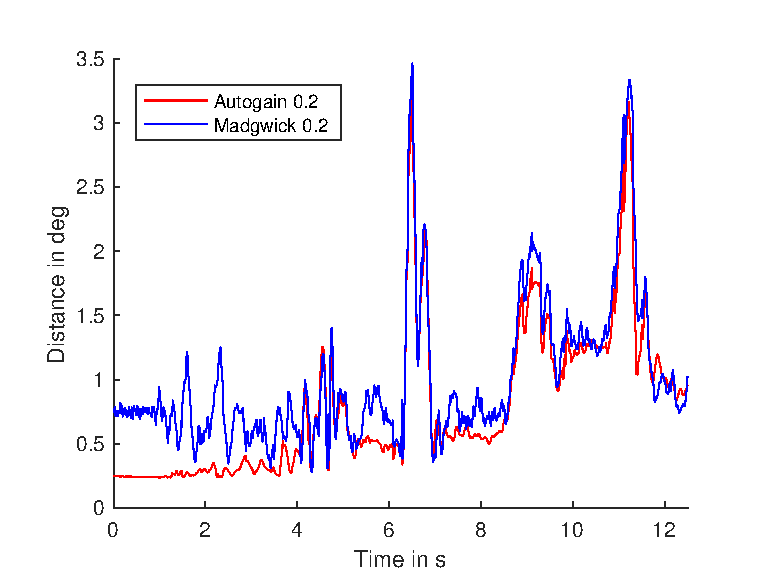
\includegraphics[width=\linewidth]{./graphics/distance.eps}
\caption{Distance of the proposed and the Madgwick algorithm to the optical tracking system, using the distance definition of \cite{kuffner2004effectiveDistance}.}
\label{distance}
\end{figure}

\begin{figure}
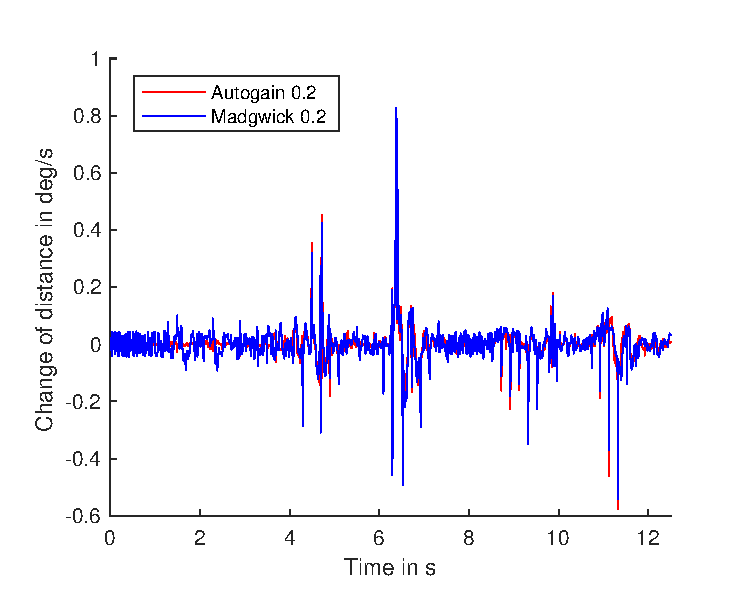
\includegraphics[width=\linewidth]{./graphics/diffdistance.eps}
\caption{Derivative of the distance of the proposed and the Madgwick algorithm to the optical tracking system, using the distance definition of \cite{kuffner2004effectiveDistance}.}
\label{diffdistance}
\end{figure}


\subsection{Position}
The primary evaluation for the position focuses on slip- and slide-behavior.
Here the plate with the IMU(s) is fixed inside a sphere with a diameter of 29 cm and rolled along an ``L''-shaped track of one meter by one meter.
Slip behavior was manually provoked.
Figure \ref{LTest} shows the resulting trajectories.
Pure rotation integration leads to an enlarged ``L'' by about 50 percent, as the manually provoked rotation is just integrated and therefore interpreted as linear motion.
The fusion between the accelerometer and gyroscope interprets an ``L'' with dimensions much closer to the original.
The estimation leaves room for improvement, as in one direction, it misses the actual length about -10 percent, and in the other direction overestimates it by 10 percent.
But it shows the overall capability of the algorithm to compensate for slip. 

\begin{figure}
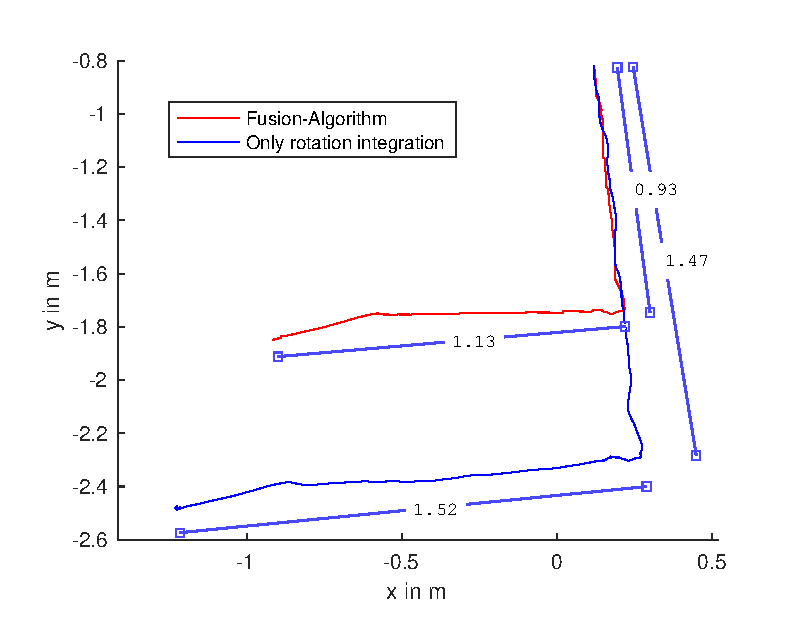
\includegraphics[width=\linewidth]{./graphics/LTest.eps}
\caption{Ground position (Z-axis, perpendicular to the ground) by integration of rotation and the fusion algorithm. An L-shape with \unit[1]{m} by \unit[1]{m} was performed with provoked slip (rotation without translation). For references the boxes are manually set points with the distance in meter between these points written on the lines connecting them. The rolling started in the upper right corner and ended in the bottom left corner. }
\label{LTest}
\end{figure}

The same experiment was performed with added slide, i.e., more translation than just the rotation produces.
Here the results shown in Figure \ref{LTestSlide} were not as reliably good as with the slip experiment.
This is due to the timing of the acceleration. In order to recognize the acceleration as translation, the rotation needs to be above a certain threshold, as the algorithm does not allow any translation without rotation at all.
The translation is computed using the accelerometer via double integration.
Therefore the acceleration of the slide movement needs to be at the same time as a minimal amount of rotation. 
If the rotation starts after the sliding, the double integration of the acceleration is suppressed.
When the rotation starts and the translation could be double integrated, it is already zero as the velocity is constant.
This can be seen in Figure \ref{LTestSlide} where the one side of the L was interpreted exactly as long as the pure integration, i.e., approx. \unit[50]{cm}, and therefore the slide was not recognized, and the other part was correctly interpreted longer than just the integration and with \unit[1.02]{m} as long as the actual trajectory.
This is to be blamed on the execution of the experiment, as it was not perfectly ensured only to start sliding with ongoing rotation, which is hard to achieve when manually guiding a sphere.
However, the sliding behavior in a real environment could be in both ways, too, so sliding while rolling and starting sliding before rolling.
With slip, this is not a problem, as, by definition, the translation cannot begin before the rotation when slipping.
If so, it would be sliding.
\begin{figure}
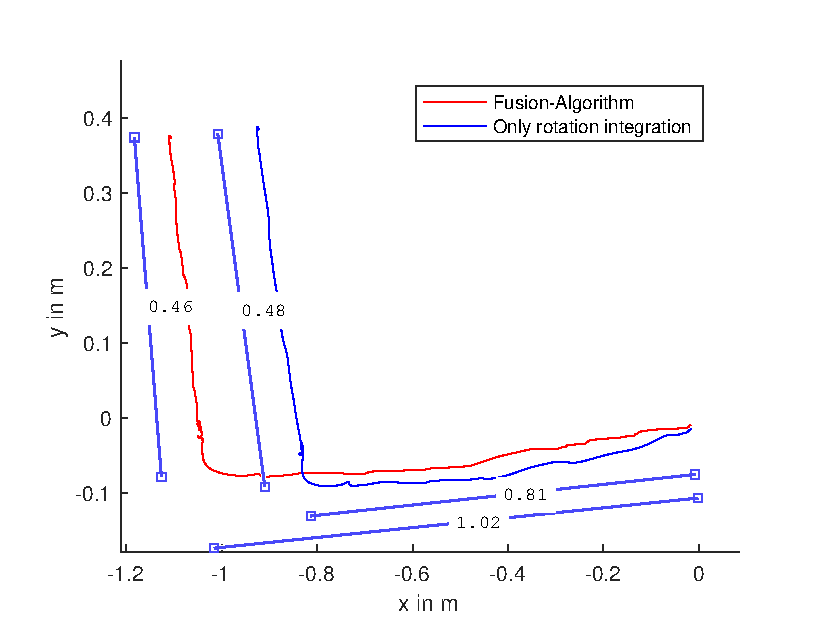
\includegraphics[width=\linewidth]{./graphics/LTestSlide.eps}
\caption{Ground position (Z-axis, perpendicular to the ground) by integration of rotation and the fusion algorithm. An L-shape with \unit[1]{m} by \unit[1]{m} was performed with provoked slide(translation without rotation). For reference the boxes are manually set points with the distance in meter between these points written on the lines connecting them. The rolling started in the lower right corner and ended in the upper left corner.}
\label{LTestSlide}
\end{figure}
The experiments for sliding did not reliably detect the slide event and, on some occasions, interpreted the distance as shorter than just the integration, as the acceleration of the linear motion was missed.
However, the deceleration of the sphere was still recognized while rotation existed, and therefore, the sphere miscalculated a couple of centimeters.


\subsection{Impact on 3D mapping}

\begin{figure}
%\begin{center}
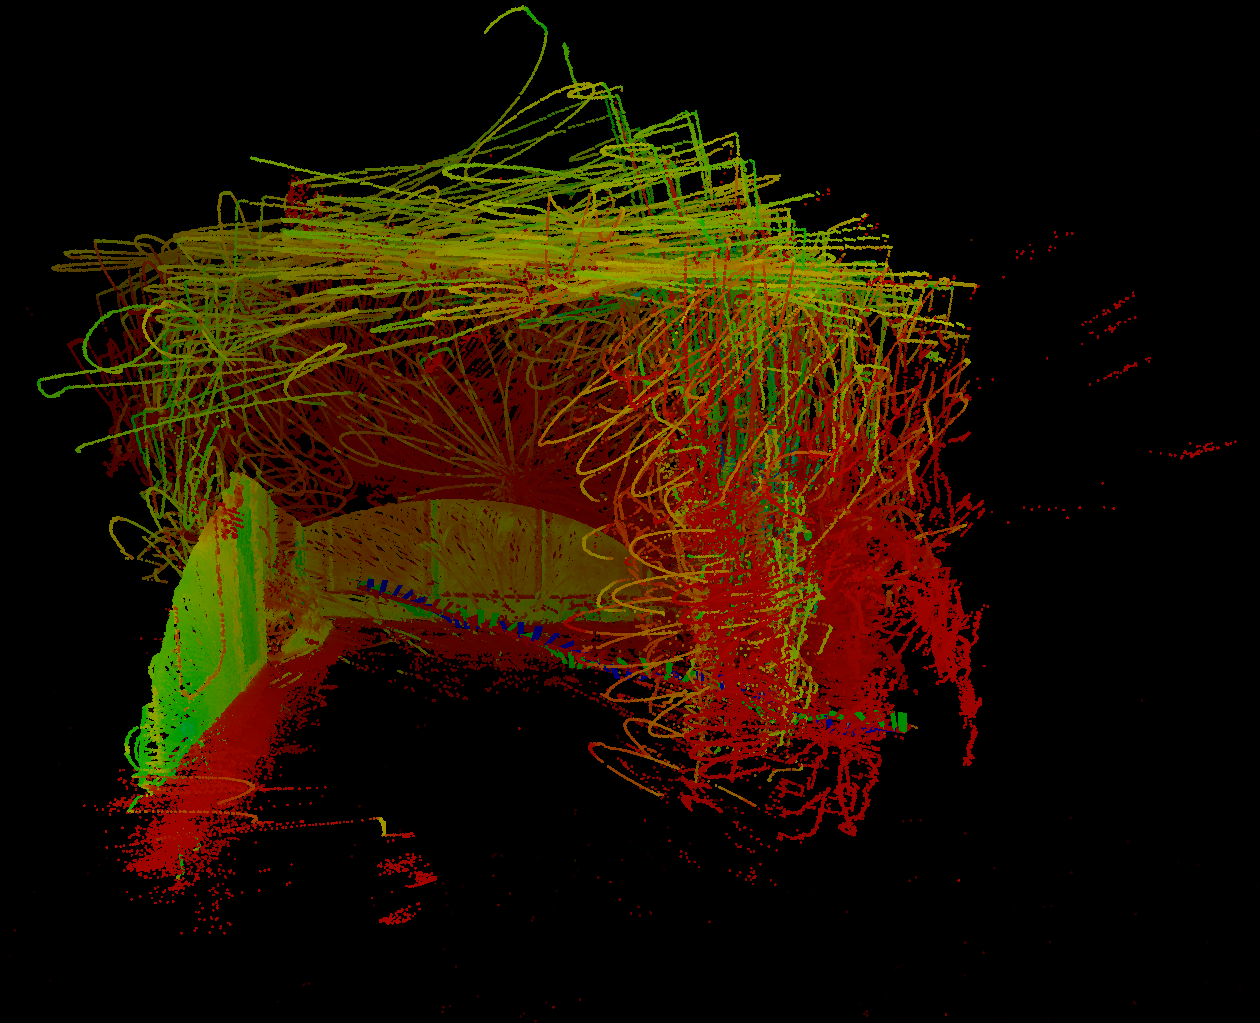
\includegraphics[width=0.52\linewidth]{./graphics/jasperhome1.png} 
%\vspace{0.2cm}
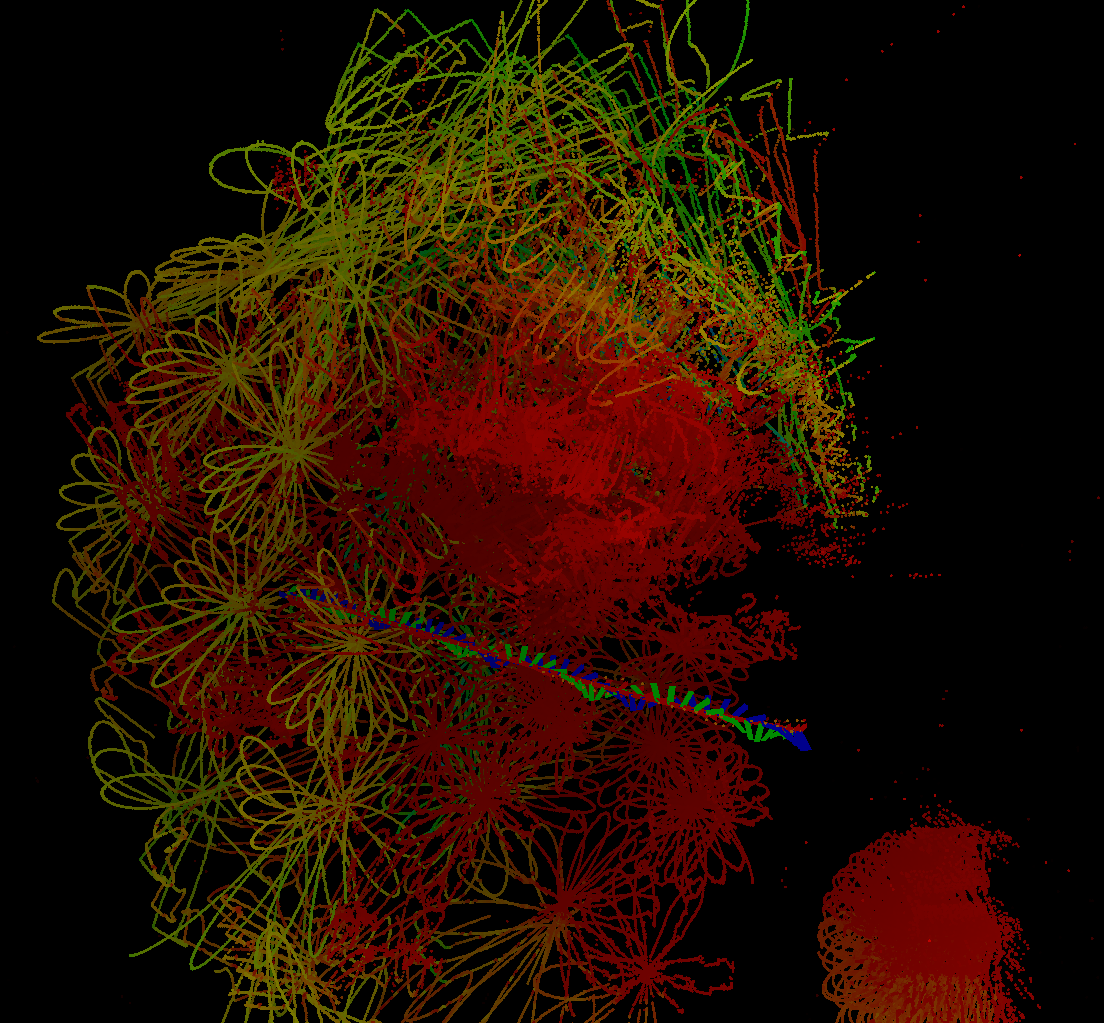
\includegraphics[width=0.45\linewidth]{./graphics/jasperhome1madw.png}
\caption{Left: resulting 3D map using the presented algorithm for pose filtering. Right: resulting 3D map using Madgwick + double integrator for pose filtering. Both images were shot from the exact same point of view. Both plots use the same LIDAR data and apply one of the simultaneously generated pose estimations.}
\label{fig:mapping}
%\end{center}
\end{figure}

One major design driver for the presented algorithm is the suitability for spherical SLAM purposes.
Therefore, a pose estimate is preferred to be slightly wrong, if it is more continuous, i.e. less noisy and with less jumping values, than the exact pose has.

To test the impact of the filter on 3D mapping, we used the prototype in Figure \ref{fig:prototype}.
After \unit[2]{s} of initial standstill, the sphere rolled approx. \unit[4]{m} within \unit[5]{s} in an indoor environment from one corner of the room to the opposing one.
We extracted the laserscan data, as well as the filtered pose using the presented algorithm.
Without further pre- or post-processing, the pose data is combined with the laserscan data to create a 3D map.
Figure \ref{fig:mapping} compares the result with another 3D map, using the pose estimation by the Madgwick filter and simple rotation integration on the same data.
Therefore the same laserscan data is mapped with different pose estimates.
The presented filter improves the resulting map compared to the Madgwick/integrator approach.
In particular, the walls and the ceiling are more recognizable, which is favorable for many SLAM algorithms.
Another improvement is that points were no longer sensed below the ground, i.e. the plane on which the sphere was moving on.
The more detailed part of the map, as seen in the bottom left corner of the above image of Figure \ref{fig:mapping}, corresponds to the initial standstill.
It is more detailed than the rest of the map because of the non-repeating flower-shaped scanning pattern, where point density increases with time.
Note that the same detailed part is also present in the right image.
However, it is out of view (at the bottom right corner) as the Madgwick filter misses the initial pose estimation by a lot. 


\subsection{Conclusion}
This paper introduced an IMU-based pose estimation filter based on the fusion of multiple already existing filters and approaches.
It is optimized for specific needs and circumstances of spherical robots with laser scanning tasks in a space-suitable way.
Needless to say, a lot of work remains to be done.
The fusion of complementary and Madgwick orientation filter solves the shortcomings of the Madgwick filter when at a standstill, particularly the jitter.
A first qualitative evaluation shows the functionality of the filter.
In further experiments, a quantitative orientation comparison with a synchronized optical system needs to be performed.
Also, as further work, all puzzle pieces, this filter, a locomotion system, a scanning system need to be combined to an overall working prototype.

The presented position estimation shows the capability to overcome the problem of the missing absolute reference of IMUs partly.
It mainly improves the measurements in the ground plane with slip behavior present.
Still, there is a need for parameter tuning. 
Sliding was not all the time detected reliably.
Here a mechanism for a delayed rotation needs to be investigated, that acceleration shortly before a rotation is integrated and taken into account once rotation starts.
The approach for, at least roughly, indicating the change in the $z$-direction, which is now done only by the accelerometer values, shows no promising results nor usable results in first qualitative experiments with rolling over obstacles and therefore needs to be re-investigated.




\addtolength{\textheight}{-12cm}   % This command serves to balance the column lengths
                                  % on the last page of the document manually. It shortens
                                  % the textheight of the last page by a suitable amount.
                                  % This command does not take effect until the next page
                                  % so it should come on the page before the last. Make
                                  % sure that you do not shorten the textheight too much.

%%%%%%%%%%%%%%%%%%%%%%%%%%%%%%%%%%%%%%%%%%%%%%%%%%%%%%%%%%%%%%%%%%%%%%%%%%%%%%%%



%%%%%%%%%%%%%%%%%%%%%%%%%%%%%%%%%%%%%%%%%%%%%%%%%%%%%%%%%%%%%%%%%%%%%%%%%%%%%%%%



%%%%%%%%%%%%%%%%%%%%%%%%%%%%%%%%%%%%%%%%%%%%%%%%%%%%%%%%%%%%%%%%%%%%%%%%%%%%%%%%







%%%%%%%%%%%%%%%%%%%%%%%%%%%%%%%%%%%%%%%%%%%%%%%%%%%%%%%%%%%%%%%%%%%%%%%%%%%%%%%%



\bibliographystyle{unsrt}
\bibliography{bibliographyJasper}


\end{document}
